\documentclass{standalone}
\usepackage{pgfplots}
\usepackage{xcolor}
\pgfplotsset{compat=1.18}

\begin{document}
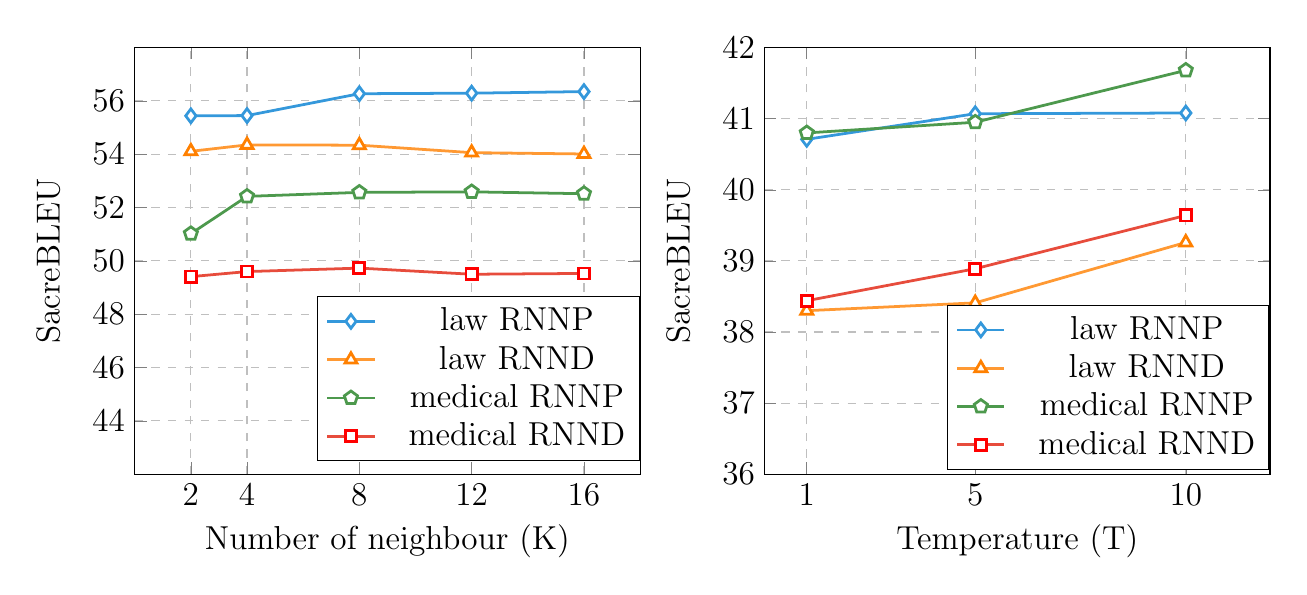
\begin{tikzpicture}

\definecolor{upurple}{RGB}{155,89,182}
\definecolor{ublue}{RGB}{52,152,219}
\definecolor{ured}{RGB}{231,76,60}
\definecolor{udark}{RGB}{77,153,77}
\definecolor{ugreen}{RGB}{46,204,113}

% 左侧图表
\begin{axis}[
name=plot1,
at={(-4cm,0)},
width=8cm,
height=7cm,
ymajorgrids,
xmajorgrids,
grid style=dashed,
legend style={
at={(0.68,0.03)},
anchor=south,
legend columns=1,
column sep=2.27ex,
font={\large},
},
xlabel={\large Number of neighbour (K)},
ylabel={\large SacreBLEU},
ylabel style={yshift=0.5em},
xlabel style={yshift=0em},
ymin=42, ymax=58,
ytick={42,44,46,48,50,52,54,56,58},
yticklabels={,44,46,48,50,52,54,56,},
xmin=0, xmax=18,
xtick={2,4,8,12,16,18},
xticklabels={2,4,8,12,16,},
xticklabel style={font={\large}},
yticklabel style={font={\large}}
]

\addplot[ublue,mark=diamond*,mark size=2.5pt,line width=1pt,mark options={fill=white,draw=ublue,line width=1pt}]
coordinates {(2,55.44) (4,55.45) (8,56.27) (12,56.29) (16,56.35)};
\addlegendentry{law RNNP}

\addplot[orange!80,mark=triangle*,mark size=2.5pt,line width=1pt,mark options={fill=white,draw=orange,line width=1pt}]
coordinates {(2,54.11) (4,54.35) (8,54.34) (12,54.06) (16,54.01)};
\addlegendentry{law RNND}

\addplot[udark,mark=pentagon*,mark size=2.5pt,line width=1pt,mark options={fill=white,draw=udark,line width=1pt}]
coordinates {(2,51.02) (4,52.42) (8,52.57) (12,52.59) (16,52.52)};
\addlegendentry{medical RNNP}

\addplot[ured,mark=square*,mark size=2pt,line width=1pt,mark options={fill=white,draw=red,line width=1pt}]
coordinates {(2,49.41) (4,49.6) (8,49.73) (12,49.5) (16,49.53)};
\addlegendentry{medical RNND}

\end{axis}

% 右侧图表
\begin{axis}[
name=plot2,
at={(4cm,0)},
width=8cm,
height=7cm,
ymajorgrids,
xmajorgrids,
grid style=dashed,
legend style={
at={(0.68,0.01)},
anchor=south,
legend columns=1,
column sep=2.27ex,
font={\large},
},
xlabel={\large Temperature (T)},
ylabel={\large SacreBLEU},
ylabel style={yshift=0.5em},
xlabel style={yshift=0em},
ymin=36, ymax=42,
ytick={36,37,38,39,40,41,42},
yticklabels={36,37,38,39,40,41,42},
xmin=0, xmax=12,
xtick={1,5,10,12},
xticklabels={1,5,10},
xticklabel style={font={\large}},
yticklabel style={font={\large}}
]

\addplot[ublue,mark=diamond*,mark size=2.5pt,line width=1pt,mark options={fill=white,draw=ublue,line width=1pt}]
coordinates {(1,40.71) (5,41.07) (10,41.08)};
\addlegendentry{law RNNP}

\addplot[orange!80,mark=triangle*,mark size=2.5pt,line width=1pt,mark options={fill=white,draw=orange,line width=1pt}]
coordinates {(1,38.3) (5,38.41) (10,39.26)};
\addlegendentry{law RNND}

\addplot[udark,mark=pentagon*,mark size=2.5pt,line width=1pt,mark options={fill=white,draw=udark,line width=1pt}]
coordinates {(1,40.8) (5,40.95) (10,41.68)};
\addlegendentry{medical RNNP}

\addplot[ured,mark=square*,mark size=2pt,line width=1pt,mark options={fill=white,draw=red,line width=1pt}]
coordinates {(1,38.44) (5,38.89) (10,39.64)};
\addlegendentry{medical RNND}

\end{axis}

\end{tikzpicture}
\end{document}